\documentclass{beamer} % [handout] para imprimir eliminando transiciones

%\usefonttheme[onlymath]{serif}
%\usepackage{fontspec}
%\defaultfontfeatures{Mapping=tex-text}
%\setsansfont[Ligatures={Common}]{Futura}
%\setmonofont[Scale=0.8]{Monaco} 

\usepackage{beamerthemesplit}
\usepackage[utf8]{inputenc}
\usepackage[spanish]{babel}
\mode<presentation>
\usetheme{default}
\usecolortheme{dolphin}
\usepackage{alltt}    % \begin{alltt}
\usepackage{amssymb}  % mathematical symbols
\usepackage{comment}
\usepackage{multicol} % \multicols
\usepackage{tabto}    % \tabto
\usepackage{verbatim} % comentarios

\title{Estructuras de datos}   %[titulo corto]
\author{Fabián Riquelme Csori} %[nombre corto]
\date{2017}                    %[fecha corta]
\institute{Universidad de Valparaíso}                 %[instituto corto]

\newcommand{\HRule}{\rule{\linewidth}{0.2mm}\\[1ex]}
\newcommand{\blue}[1]{\textcolor{blue}{#1}}
\newcommand{\red}[1]{\textcolor{red}{#1}}
\newcommand{\redb}[1]{{\color{red!70!black}{#1}}}
\newcommand{\green}[1]{{\color{green!70!black}{#1}}}
\newcommand{\gray}[1]{{\color{gray!50!white}{#1}}}
\newcommand{\textgreek}[1]{\begingroup\fontencoding{LGR}\selectfont#1\endgroup}
% \alert{texto destacado en rojo}
% \color{green} Color en verde
% \structure{texto en lila}

\begin{document}


%\begin{frame}%[plain]
%  \titlepage
%\end{frame}
%
% [opciones]:
% plain: oculta barra de navegacion, deja + espacio para contenido
% fragile: usar comandos como verbatim
% b,c,t: alineacion vertical
% label=nombre_etiqueta
% allowframebreaks: divide contenido en varios frames si es demasiado largo
% shrink: para escribir mucho texto en una transparencia, reduciendo tamano de fuente

%%%%%%%%%% PORTADA %%%%%%%%%%
\begin{frame}[plain]
  \begin{figure}[h]
    \begin{minipage}{0.3\textwidth}
    
\includegraphics[width=.9\textwidth]{./image/logo-UV.png}
    \end{minipage}
    \begin{minipage}{0.65\textwidth}
     $~$\\[3.6ex]
     \footnotesize{Escuela de Ingeniería Civil Informática}\\
     \footnotesize{Facultad de Ingeniería}
    \end{minipage}
  \end{figure}
  \begin{center}
    \vspace{1ex}
    \HRule
    \Large{Estructuras de datos}\\{\small Capítulo II: Estructuras de datos fundamentales}\\[-1ex]
    \HRule\vspace{1ex}
    \large{Fabián Riquelme Csori}\\[.5ex]\footnotesize{fabian.riquelme@uv.cl}\\[6ex] {\tiny 2017-II}\\[6ex]
  \end{center}
\end{frame}

%%%%%%%%%% INDEX %%%%%%%%%%
\begin{frame}
 \frametitle{Index}
 \scriptsize 			% reducir tamano de letra
 \tableofcontents		%[pausesections]
\end{frame}

%%%%%%%%%%% ACTUAL INDEX %%%%%%%%%%
%\AtBeginSection[] %generar indice automaticamente
%{
%\begin{frame}<beamer>%[plain]
% \frametitle{Index}
% \framesubtitle{subtitulo}
% \scriptsize
% \tableofcontents[currentsection, currentsubsection]
%\end{frame}
%}

%==============================
\section{Tipos de datos abstractos}

%------------------------------
\subsection{Elementos de un TDA}

\begin{frame}{Elementos de un TDA}
    Un \blue{tipo de datos abstracto} (\blue{TDA} o \blue{ADT}) está conformado por:
    \begin{itemize}
        \item Una \red{colección} de datos.
        \item Un conjunto de \red{operaciones} sobre los datos\\
        (o sobre un subconjunto de ellos).
        \item Un conjunto de \red{axiomas} que controlan y restringen el uso de las operaciones.
    \end{itemize}
    \pause
    Los TDA son independientes de la implementación, y permiten acceder a sus operaciones mediante una interfaz.

    \pause
    Una \blue{estructura de datos} es una implementación de un TDA.\\
    Ej: las clases \texttt{vector}, \texttt{list}, \texttt{stack}, ... de \red{C++ Standard Library}.
\end{frame}

%------------------------------
\subsection{Notación de un TDA}

\begin{frame}{Notación de un TDA}
    No existe una notación estándar para describir un TDA.
    
    Una notación posible puede ser:
    \medskip
    
    \begin{tabular}{lp{45ex}}\hline
      {\bf ADT\_name}   & {\small Breve descripción de la colección de datos.}\\
      {\bf Operations} & {\small Lista de operaciones, con parámetros de entrada entre paréntesis, más breves descripciones.}\\
      {\bf Axioms}     & {\small Definidos lo más formalmente posible en términos de las operaciones.}\\\hline
    \end{tabular}
    \medskip
    
    \footnotesize{
    \begin{itemize}
        \item<2-> El detalle de las operaciones se puede describir con pseudocódigo aquí o después de los axiomas, indicando la salida (output).
        \item<3-> Los axiomas pueden ser (in)consistentes y (in)completos.\\
        Un conjunto de axiomas completo puede tener axiomas redundantes.
        \item<4-> Es bueno incluir además la complejidad computacional de cada operación.
        \item<5-> En adelante omitiremos operaciones de constructores y destructores.
    \end{itemize}}
\end{frame}

%==============================
\section{Vectores, pilas y colas}

%------------------------------
\subsection{Vectores}

\begin{frame}{Vector}
    \begin{itemize}
        \item A diferencia de un \blue{\texttt{array}}, posee un tamaño variable.
        \item A cambio, su rendimiento es ligeramente inferior (punteros).\\
        \item Aún así, salvo para arreglos muy pequeños cuyo contenido debe modificarse constantemente, es preferible usar una estructura de datos \blue{\texttt{vector}} por sobre los arreglos.
    \end{itemize}
    \begin{center}
        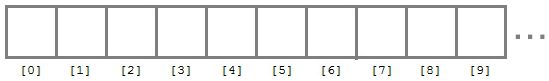
\includegraphics[width=.8\textwidth]{./image/cap2/vector.png}
    \end{center}
    \pause
    
    {\small Nota: Python al definir ``\texttt{var=[a,b]}'' en realidad usa su clase \texttt{list}.\\
    Para este lenguaje existe el paquete \red{NumPy} que utiliza arreglos multi-dimensionales eficientes.}
\end{frame}

\begin{frame}{Vector: TDA}
    \scriptsize{
    \begin{tabular}{lp{60ex}}\hline\\[-1ex]
      {\bf\normalsize vector} & Sequential, random-access, variable-size elements container (of the same type).\\
      {\bf\small operations}  & \\
      size()            & How many elements are in the collection?\\
      isEmpty()         & Is the collection empty?\\
      contains(element) & Does the collection contain the given element?\\
      elementAt(index)  & Access the element at the given index.\\
      clear()           & Make the collection empty.\\
      append(element)   & Add a new element to the end of the collection.\\
      insertAt(index, element) & Insert a new element at the given index.\\
      remove(element)   & Remove the given element from the collection.\\
      removeAt(index)   & Remove the element at the given index.\\
      replace(index, element) & Replace the element at the given index with a new element.\\[1.5ex]\hline
    \end{tabular}

    \begin{itemize}
        \item<2-> ¿Cuál sería el output de cada operación?
        \item<3-> ¿Qué operadores son de capacidad, acceso, modificadores, comparadores?
    \end{itemize}}
\end{frame}

\begin{frame}{Vector: TDA}
    \scriptsize{
    Sea $n$ el tamaño de un vector y $n'$ su tamaño luego de modificarse:
    \medskip
    
    \begin{tabular}{lp{60ex}}\hline
      {\bf Operación}   & {\bf Complejidad}\\\hline
      size()            & $O(1)$\\
      isEmpty()         & $O(1)$\\
      contains(element) & $O(n)$\\
      elementAt(index)  & $O(1)$\\
      clear()           & $O(n)$\\
      append(element)   & $O(1)$; $O(n')$ si hay reasignación de memoria\\
      insertAt(index, element) & $O(m)\leq O(n)$; $m$ son los elementos desde index+1\\
      remove(element)   & $O(n)$ en el peor caso\\
      removeAt(index)   & $O(m)\leq O(n)$; $m$ son elementos después de los borrados\\
      replace(index, element) & $O(1)$\\[1.5ex]\hline
    \end{tabular}

    \begin{itemize}
        \item<2-> ¿Qué complejidad tendría una operación       indexOf(element), que retorna el índice de un elemento dado?
    \end{itemize}}
\end{frame}

\begin{frame}{Vector: TDA}
    \scriptsize{
    \begin{tabular}{p{87ex}}\hline\\[-1ex]
      {\bf\normalsize axioms}\\
      For any vector $V$, element $a$, index $i$, integer $n$:\\[1.2ex]
      1. V.size(), V.isEmpty(), V.contains(a), V.clear() and V.append(a) are always defined\\
      2. (V.append(a)).isEmpty() = false\\
      3. (V.append(a)).size() = V.size()+1\\
      4. (V.insertAt(i,a)).size() = V.size()+1\\
      5. (V.remove(a)).size() $\leq$ V.size()\\
      6. (V.removeAt(i)).size() = V.size()-1\\
      7. (V.insertAt(i,a)).removeAt(i) = V\\
      8. (V.insertAt(i,a)).elementAt(i) = a\\[1.5ex]\hline
    \end{tabular}

    \begin{itemize}
        \item<2-> Este conjunto de axiomas es consistente. ¿Será completo? ¿será redundante?
        \item<3-> Verificar qué operaciones están implementadas en la estructura de datos \texttt{vector} de la C++ Standard Library, y cuáles no: \url{http://www.cplusplus.com/reference/vector/vector/}
        \item<4-> Ejercicio: Definir nuevos axiomas, e implementar las operaciones que falten.
    \end{itemize}}
\end{frame}


%------------------------------
\subsection{Pilas}

\begin{frame}{Pila/Stack}
    \begin{itemize}
        \item<1-> Como el vector, es una estructura secuencial y de tamaño variable, pero donde solo se puede agregar o quitar elementos desde uno de sus extremos.
        \item<2-> Los elementos se eliminan en el orden inverso al que se insertaron $\to$ estructura \blue{LIFO} (last-in, first-out).
        \smallskip
        
        \begin{center}
            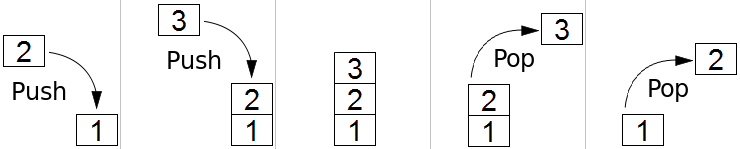
\includegraphics[width=.8\textwidth]{./image/cap2/stack.png}
        \end{center}
        \item<3-> ¿Aplicaciones? \uncover<4->{Cadenas de producción, análisis sintáctico, programación lógica, etc.}
        \item<5-> El \blue{tope} es el único elemento visible, i.e., el último agregado.
    \end{itemize}
\end{frame}

\begin{frame}{Pila/Stack: errores usuales}
    \begin{itemize}
        \item<1-> Una pila, como un vector, puede definirse con un tamaño máximo. Si se agregan más elementos que este máximo, se produce un error conocido como \blue{desbordamiento} u \blue{overflow}.
        \begin{itemize}
            \item<2-> Para evitar overflow sin usar un máximo muy grande se pueden definir pilas con espacio compartido:\\[1.5ex]
            \begin{center}
                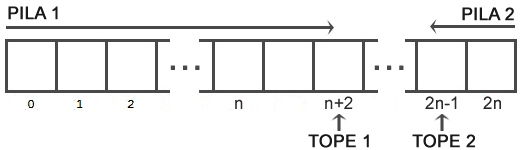
\includegraphics[width=.8\textwidth]{./image/cap2/stacks-sharing.png}
            \end{center}
        \end{itemize}
        \item<3-> Al contrario, si se intenta quitar un elemento de una pila vacía, se produce un error de \blue{subdesbordamiento} o \blue{underflow}.
    \end{itemize}
\end{frame}

\begin{frame}{Pila/Stack: TDA}
    \scriptsize{
    \begin{tabular}{lp{60ex}}\hline\\[-1ex]
      {\bf\normalsize stack} & LIFO, variable-size elements container (of the same type).\\[1.5ex]
      {\bf\small operations}  & \\
      size()            & How many elements are in the stack?\\
      isEmpty()         & Is the stack empty?\\
      top()             & Access the element at the top of the stack.\\
      push(element)     & Add a new element at the top of the stack.\\
      pop()             & Remove the top element of the stack.\\[1.5ex]\hline
    \end{tabular}

    \begin{itemize}
        \item<2-> ¿Cuál sería el output de cada operación?
        \item<2-> ¿Qué operadores son de capacidad, acceso, modificadores, comparadores?
    \end{itemize}}
\end{frame}

\begin{frame}{Pila/Stack: TDA}
    \scriptsize{
    \begin{center}
    \begin{tabular}{lc}\hline
      {\bf Operación}   & {\bf Complejidad}\\\hline
      size()            & $O(1)$\\
      isEmpty()         & $O(1)$\\
      top()             & $O(1)$\\
      push(element)     & $O(1)$\\
      pop()             & $O(1)$\\[1.5ex]\hline
    \end{tabular}
    \end{center}}
\end{frame}

\begin{frame}{Pila/Stack: TDA}
    \scriptsize{
    \begin{tabular}{p{87ex}}\hline\\[-1ex]
      {\bf\normalsize axioms}\\
      For any stack $S$, element $a$:\\[1.2ex]
      1. S.size(), S.IsEmpty(), S.push(a) are always defined\\
      2. If (S.isEmpty() = true) then (S.top( ) = error)\\
      3. If (S.isEmpty() = true) then (S.pop( ) = error)\\
      4. (S.push(a)).isEmpty() = false\\
      5. (S.push(a)).top( ) = a\\
      6. (S.push(a)).pop( ) = S\\[1.5ex]\hline
    \end{tabular}

    \begin{itemize}
        \item<2-> Verificar operaciones implementadas en estructura de datos \texttt{stack} de C++ Standard Library: \url{http://www.cplusplus.com/reference/stack/stack/}
        \item<2-> Ejercicio: Definir nuevos axiomas (puede utilizar operaciones de constructores).
    \end{itemize}}
\end{frame}

%------------------------------
\subsection{Colas}

\begin{frame}{Cola/Fila/Queue}
    \begin{itemize}
        \item<1-> Como las anteriores, es una estructura secuencial y de tamaño variable, pero donde solo se puede agregar por un extremo y quitar por el otro.
        \item<2-> Los elementos se eliminan en el mismo orden en el que se insertaron $\to$ estructura \blue{FIFO} (first-in, first-out).
        \smallskip
        
        \begin{center}
            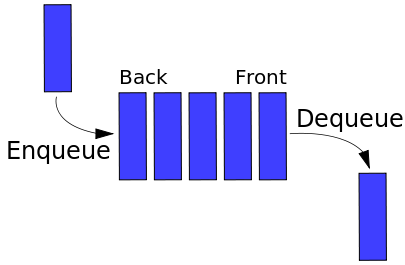
\includegraphics[width=.5\textwidth]{./image/cap2/queue.png}
        \end{center}
        \item<3-> ¿Aplicaciones? \uncover<4->{Cadenas de producción, listas de espera en sistemas operativos, etc.}
    \end{itemize}
\end{frame}


\begin{frame}{Cola/Fila/Queue: TDA}
    \scriptsize{
    \begin{tabular}{lp{60ex}}\hline\\[-1ex]
      {\bf\normalsize queue} & FIFO, variable-size elements container (of the same type).\\[1.5ex]
      {\bf\small operations}  & \\
      size()            & How many elements are in the queue?\\
      isEmpty()         & Is the queue empty?\\
      front()           & Access the element at the front of the queue.\\
      push(element)     & Add a new element at the back of the queue.\\
      pop()             & Remove the element at the front of the queue. \\[1.5ex]\hline
    \end{tabular}

    \begin{itemize}
        \item<2-> ¿Cuál sería el output de cada operación?
        \item<2-> ¿Qué operadores son de capacidad, acceso, modificadores, comparadores?
    \end{itemize}}
\end{frame}

\begin{frame}{Cola/Fila/Queue: TDA}
    \scriptsize{
    \begin{center}
    \begin{tabular}{lc}\hline
      {\bf Operación}   & {\bf Complejidad}\\\hline
      size()            & $O(1)$\\
      isEmpty()         & $O(1)$\\
      front()           & $O(1)$\\
      push(element)     & $O(1)$\\
      pop()             & $O(1)$\\[1.5ex]\hline
    \end{tabular}
    \end{center}}
\end{frame}

\begin{frame}{Cola/Fila/Queue: TDA}
    \scriptsize{
    \begin{tabular}{p{87ex}}\hline\\[-1ex]
      {\bf\normalsize axioms}\\
      For any queue $Q$, element $a$:\\[1.2ex]
      1. Q.size(), Q.IsEmpty(), Q.push(a) are always defined\\
      2. (Q.push(a)).isEmpty() = false\\
      3. If (Q.isEmpty() = true) then (Q.front( ) = error)\\
      4. If (Q.isEmpty() = true) then (Q.pop( ) = error)\\
      5. if (Q.isEmpty() = true) then (Q.push(a)).front( ) = a\\
      6. if (Q.isEmpty() = true) then (Q.push(a)).pop( ) = Q\\[1.5ex]\hline
    \end{tabular}

    \begin{itemize}
        \item<2-> Verificar operaciones implementadas en estructura de datos \texttt{queue} de C++ Standard Library: \url{http://www.cplusplus.com/reference/queue/queue/}
        \item<2-> Ejercicio: Definir nuevos axiomas (puede utilizar operaciones de constructores).
    \end{itemize}}
\end{frame}

%==============================
\section{Listas y listas enlazadas}

%------------------------------
\subsection{Listas}

\begin{frame}{Lista/List}
    \begin{itemize}
        \item Como las estructuras anteriores (vectores, pilas y colas) es un contenedor secuencial y de tamaño variable.
        \item Sus implementaciones utilizan uno o dos ``cabezales'' móviles, para recorrerla de izquierda a derecha.
        \begin{itemize}
            \item Los vectores no usan cabezales (acceso directo/aleatorio).
            \item Las pilas tienen solo un cabezal fijo en el tope.
            \item Las colas tienen un cabezal fijo en el back y otro en el front\\$\to$ este es el caso de las listas.
        \end{itemize}
    \end{itemize}
    \begin{center}
        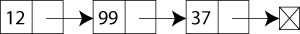
\includegraphics[width=.5\textwidth]{./image/cap2/list.png}
    \end{center}
\end{frame}

\begin{frame}{Lista/List}
    \begin{itemize}
        \item<1-> \blue{Ventajas}
        \begin{itemize}
            \item Son más eficientes en operaciones de inserción, extracción y mover elementos $\to$ de $O(n)$ en peor caso se pasa a $O(1)$.
            \item Preferibles en algoritmos que usan mucho estas operaciones, como algoritmos de ordenamiento.
        \end{itemize}
        \item<2-> \blue{Desventajas}
        \begin{itemize}
            \item No permiten acceso directo a sus elementos (para acceder a un elemento, hay que recorrer la lista desde la ubicación actual del cabezal) $\to$ de $O(1)$ se pasa a $O(n)$ en el peor caso.
            \item Usan un poco más de memoria para mantener a los elementos asociados (punteros).
            \item No recomendadas si serán listas muy grandes con elementos muy pequeños.
        \end{itemize}
    \end{itemize}
\end{frame}

\begin{frame}{Lista/List: TDA}
    \scriptsize{
    \begin{tabular}{lp{60ex}}\hline\\[-1ex]
      {\bf\normalsize list} & Sequential, variable-size elements container (of same type).\\[1.5ex]
      {\bf\small operations}  & \\
      size()            & How many elements are in the list?\\
      isEmpty()         & Is the list empty?\\
      front()           & Access the element at the front of the list.\\
      back()            & Access the element at the back of the list.\\
      get(position)     & Access the element at the given position.\\
      clear()           & Make the list empty.\\
      push\_back(element)  & Add a new element to the back of the list.\\
      push\_front(element) & Add a new element to the front of the list.\\
      insert(position, element) & Insert a new element at the given position in the list.\\
      pop\_back()       & Remove the element at the back of the list.\\
      pop\_front()      & Remove the element at the front of the list.\\
      remove(element)   & Remove the given element from the coalition. \\
      remove(position)  & Remove the element at the given position. \\[1.5ex]\hline
    \end{tabular}

    \begin{itemize}
        \item<2-> ¿Cuál sería el output de cada operación?
        \item<2-> ¿Qué operadores son de capacidad, acceso, modificadores, comparadores?
    \end{itemize}}
\end{frame}

\begin{frame}{List: TDA}
    \scriptsize{
    Sea $n$ el tamaño de un vector:

    \begin{center}
    \begin{tabular}{ll}\hline
      {\bf Operación}   & {\bf Complejidad}\\\hline
      size()            & $O(n)$\\
      isEmpty()         & $O(1)$\\
      front()           & $O(1)$\\
      back()            & $O(1)$ (con dos cabezales)\\
      get(position)     & $O(n)$\\
      clear()           & $O(n)$\\
      push\_back(element)  & $O(1)$\\
      push\_front(element) & $O(1)$\\
      insert(position, element) & $O(1)$ + search time\\
      pop\_back()       & $O(1)$\\
      pop\_front()      & $O(1)$\\
      remove(element)   & $O(n)$ en el peor caso\\
      remove(position)  & $O(1)$ + search time\\[1.5ex]\hline
    \end{tabular}
    \end{center}}
\end{frame}

\begin{frame}{Lista/List: TDA}
    \scriptsize{
    \begin{tabular}{p{87ex}}\hline\\[-1ex]
      {\bf\normalsize axioms}\\
      For any list $L$, element $a$, position $p$:\\[1.2ex]
      1. L.size(), L.isEmpty(), L.clear(), L.push\_back(a), L.push\_front(a) are always defined\\
      2. (L.push\_back(a)).IsEmpty() = false\\
      3. (L.insert(p,a)).IsEmpty() = false\\
      4. (L.push\_back(a)).size() = L.size()+1\\
      5. (L.insert(p,a)).size() = L.size()+1\\
      6. (L.pop\_back()).size() = L.size()-1\\
      7. (L.remove(a)).IsEmpty() $\leq$ L.size()\\
      8. If (L.isEmpty() = true) then (L.back() = error)\\
      9. If (L.isEmpty() = true) then (L.pop\_back() = error)\\
      10. if (L.isEmpty() = true) then (L.push\_back(a)).back() = a\\
      11. if (L.isEmpty() = true) then (L.push\_back(a)).pop\_back() = L\\
      12. (L.insert(p,a)).remove(p) = L\\
      13. L.get(p) = (L.insert(p,a)).get(p+1)\\
      14. L.get(p+1) = (L.remove(p)).get(p)\\
      idem reemplazando 'back' por 'front' donde corresponda.\\[1.5ex]\hline
    \end{tabular}

    \begin{itemize}
        \item<2-> Verificar operaciones implementadas en estructura de datos \texttt{list} de C++ Standard Library: \url{http://www.cplusplus.com/reference/list/list/}
        \item<2-> Ejercicio: Definir nuevos axiomas.
    \end{itemize}}
\end{frame}

%------------------------------
\subsection{Listas enlazadas}

\begin{frame}{Listas enlazadas}
    \begin{itemize}
        \item<1-> Una \blue{lista enlazada} es una estructura de datos, i.e., una implementación posible del TDA lista.
        \item<2-> \blue{Ventajas}
        \begin{itemize}
            \item Son estructuras dinámicas, i.e., pueden ocupar y desechar memoria en tiempo de ejecución.
            \item Inserción y eliminación están implementadas inteligentemente, y se pueden hacer en cualquier parte de la lista.
            \item Otras estructuras dinámicas como pilas y colas pueden implementarse como listas enlazadas.
            \item No necesitan definir un tamaño inicial.
        \end{itemize}
        \item<3-> \blue{Desventajas}
        \begin{itemize}
            \item Mayor uso de memoria que arreglos y vectores (punteros).
            \item Los nodos deben leerse en orden, secuencialmente.
            \item Pequeño costo asociado para acceder al contenido de un nodo.
        \end{itemize}
    \end{itemize}
\end{frame}

\begin{frame}{Operaciones}
    \begin{itemize}
        \item<1-> \blue{Insertion}
        
            \begin{center}
            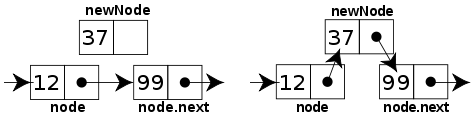
\includegraphics[width=.7\textwidth]{./image/cap2/linked-list-insertion.png}
            \end{center}
        \item<2-> \blue{Deletion}
        
            \begin{center}
            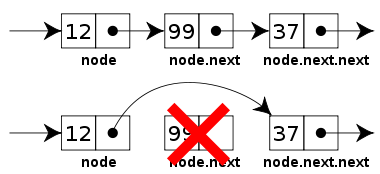
\includegraphics[width=.6\textwidth]{./image/cap2/linked-list-deletion.png}
            \end{center}
    \end{itemize}
\end{frame}

\begin{frame}{Ejercicio: Listas enlazadas}
    \begin{itemize}
        \item Implemente una lista enlazada que reciba como entrada una lista de las notas de un curso de 10 alumnos: 10 números decimales (puede restringirse a un decimal) entre 1.0 y 7.0.\\
        \small{Idealmente use C o C++, pero sin la STL o C++ Standard Library.}
        \begin{enumerate}
            \item Reordene dicha secuencia de números de menor a mayor.
            \item Copie aquellos valores de la lista que son mayores que 4.0 en otra lista enlazada, y elimínelos de la lista original.
            \item Añada entre el quinto y el sexto nodo de la primera lista enlazada un nodo adicional, cuyo valor corresponda al promedio de notas en dicha lista.
        \end{enumerate}
        \item Repita el ejercicio utilizando la clase List de C++.
    \end{itemize}
\end{frame}

\begin{frame}{Ejercicio: Vectores, Pilas y Colas}
    \begin{itemize}
        \item Utilizando la filosofía del TDA Vector, defina un TDA Matriz.
        \item Implemente dos pilas con memoria compartida.
        \item A partir de la estructura de datos Fila de algún lenguaje de programación, implemente dos operaciones:
        \begin{itemize}
            \item front2(): hace lo mismo que front(), pero no accede al primero, sino al segundo elemento encolado.
            \item pop2(): hace lo mismo que pop(), pero no elimina el primero, sino el segundo elemento encolado.
        \end{itemize}
    \end{itemize}
\end{frame}

%------------------------------

\begin{frame}
 \begin{block}{Bibliografía recomendada}
  \begin{itemize}
    \item Weiss, M., Estructura de datos y algoritmos,\\ Addison-Wesley, 1995.
    \item Aho, Hopcroft y Ullman, Estructuras de datos y algoritmos, Addison-Wesley, 1988.
  \end{itemize}
 \end{block}
 \begin{block}{Recursos}
  \begin{itemize}
    \item Wikimedia Commons.
    \item \url{http://www.cplusplus.com}
  \end{itemize}
 \end{block}
\end{frame}

\end{document}
